\documentclass[tikz, border = 1 cm]{standalone}
\usepackage{tikz}

\usepackage{tkz-euclide}
\usetikzlibrary{intersections}

\begin{document}

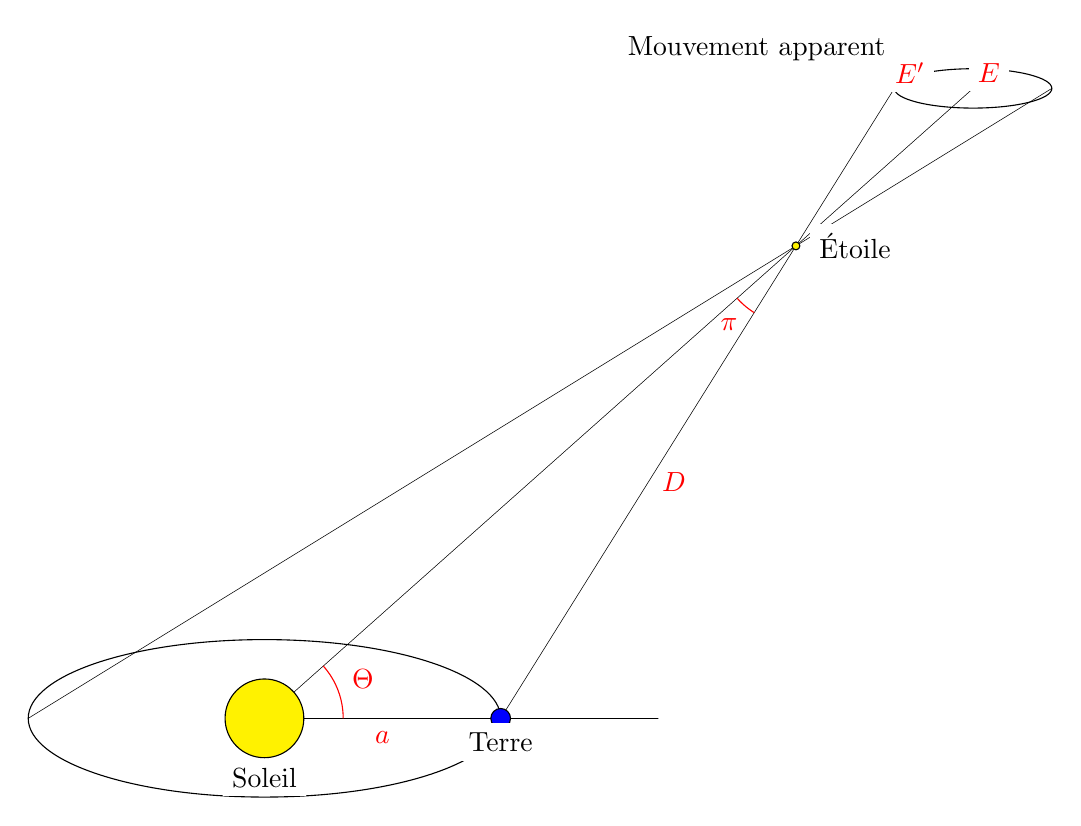
\begin{tikzpicture}
 \tkzDefPoint(0,0){A}  \tkzDefPoint(9,8){B}
  \tkzDefPoint(3,0){C}  \tkzDefPoint(8,8){D}
  \tkzDefPoint(5,0){F}
  \tkzDefPoint(-3,0){G} \tkzDefPoint(10,8){H}
  \tkzDrawSegments(A,B C,D)
  \tkzDrawSegments(A,F)
  \tkzDrawSegments(G,H)
  \tkzInterLL(A,B)(C,D) \tkzGetPoint{E}
  \tkzDrawPoints(E)

      \filldraw[fill=yellow] (E) circle (0.05);
      \filldraw[fill=yellow] (A) circle (0.5);
      \draw (A) ellipse (3 and 1);
      \filldraw[fill=blue] (C) circle (0.125);
      \draw (B) ellipse (1 and 0.25);

      \begin{scope}
        % pour limiter la portée du \clip
        \clip (A) -- (E) -- (C) -- cycle; % triangle AEC
        \draw [red] (A) circle (1);
        \draw [red] (E) circle (1);
      %  \draw [red] (C) circle (1);
        % cercle pour arc
      \end{scope}

      
      \node[red] at (1.25,0.5) {$\Theta$};
      \node[red] at (5.9,5) {$\pi$};
      \node[red] at (5.2,3) {$D$};
      \node[red] at (1.5,-0.250) {$a$};
      
      \node[fill=white] at (3,-0.3) {Terre};
      \node[fill=white] at (0,-0.75) {Soleil};
      \node[fill=white] at (6.25,8.5) {Mouvement apparent};
      \node[fill=white] at (7.5,6) {\'Etoile};
      \node[red,fill=white] at (8.2,8.2) {$E'$};
      \node[red,fill=white] at (9.2,8.2) {$E$};
\end{tikzpicture}

\end{document}
